\documentclass[11pt]{article}
\usepackage{hyperref}
\usepackage[english]{babel}
\usepackage{blindtext}
\usepackage{url}
\usepackage{graphicx}
\usepackage{multicol}
\usepackage[center]{titlesec}
\usepackage{geometry}
%\usepackage{mathtools}

\usepackage[sort, numbers]{natbib}


%
%\setlength{\columnseprule}{0.4pt}
%\setlength{\footskip}{20pt}
\usepackage{fancyhdr}
\fancyhf{}
\fancyhead[C]{PHC 6016 $\bullet$ Joe Brew $\bullet$ Social Epidemiology}
\fancyfoot[C]{  $\bullet$ Assignment 3 \bullet$  }
\renewcommand\headrulewidth{1pt}
\renewcommand\footrulewidth{1pt}
\pagestyle{fancy}

%

\setlength{\columnsep}{1.5cm}
%\setlength{\columnseprule}{0.4pt}

%\MakeOuterQuote{"}



\graphicspath{ {/home/joebrew/Documents/uf/phc6016/assignment4} }

%the next two lines adjust the third, centered section of the exec sum
\def\changemargin#1#2{\list{}{\rightmargin#2\leftmargin#1}\item[]}
\let\endchangemargin=\endlist 

\usepackage{Sweave}
\begin{document}
\Sconcordance{concordance:global_variance.tex:global_variance.Rnw:%
1 40 1 1 0 24 1 1 44 1 1 1 90 24 1 1 17 1 2 4 1 1 17 1 2 9 1 1 10 1 4 8 %
1 1 21 1 3 8 1 1 20 1 2 10 1 1 23 1 3 5 1 1 32 1 2 23 1 1 24 1 3 6 1 1 %
29 1 3 19 1}


\title{\textbf{Global variance in childhood obesity}}
\author{Joe Brew}


\maketitle

\emph{
Discuss the global variance in the public health problem you choose.  Are there particular reasons to study the problem in particular places, for instance where exposure is earlier, or untreated prevalence is higher, or incidence is especially high? I am especially interested in you find out if  relationships differ in other places.  For instance, a region where gonorrhea is high and the quality of the neighborhood is low.  This would mean this is an interesting place to study "your" problem.
}
\tableofcontents

\vspace{20mm}

\begin{center}

\includegraphics[width=2cm]{uf}
\end{center}


\newgeometry{margin=2.5cm}
\fancyhfoffset[E,O]{0pt}




%------------------------------------------
\section*{Assignment 3}
\addcontentsline{toc}{section}{Assignment 3}
%------------------------------------------
\hrulefill

\begin{multicols}{2} 
\setkeys{Gin}{width=0.45\textwidth}

%------------------------------------------
\subsection*{Background}
\addcontentsline{toc}{subsection}{Background}
%------------------------------------------

Pediatric adiposity is one of the public health measures with the most global variance.  Though the prevalence of childhood obesity and overweight (like adult obesity and overweight) is increasing rapidly in most developing countries (and shows no signs of decline in developed countries), variations in both the rate of increase and the "take-off" time (ie, the moment at which the increase began) have lead to a massively unequal distribution of childhood obesity throughout the world.  \\

The prevalence of childhood obesity varies by socioeconomic class, race, geography, time and numerous other factors.  For the purposes of this (short) paper, I examine the prevalence of childhood overweight (limited here to children 2-4 years of age only) at the \emph{country} level.  The raw data used for the following analysis come from the WHO, IMF and OECD, but all figures and calculations (and the errors therein) are entirely mine. \\

%------------------------------------------
\subsection*{Variance}
\addcontentsline{toc}{subsection}{Variance}
%------------------------------------------
At the country level, the mean prevalence of childhood overweight is 7.51\%, with a standard deviation of 4.78\%.  The distribution ranges from approximately 0\% (North Korea, according to the WHO) to 23.4\% (Albania), and can be visualized below.\\

\begin{center}
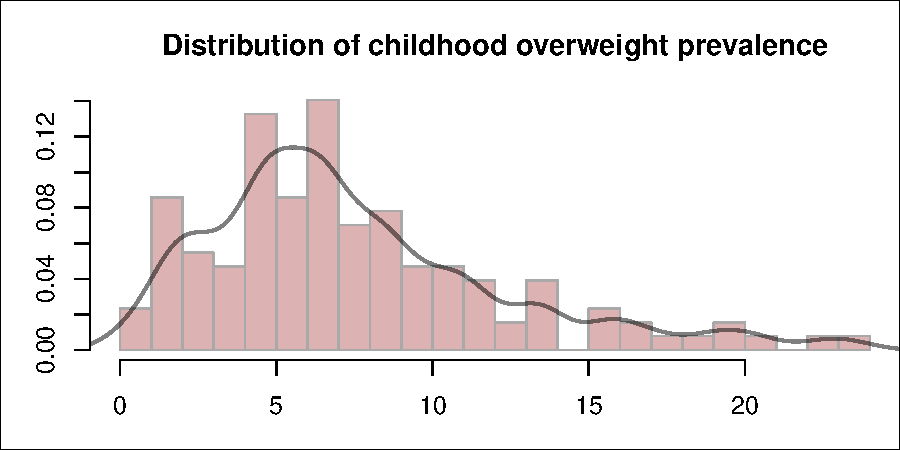
\includegraphics{global_variance-003}
\end{center}

Though slightly right-skewed, the global distribution is remarkably normal (gaussian), a fact which differentiates it from the global distribution of the prevalence of childhood underweight (below).\\

\begin{center}
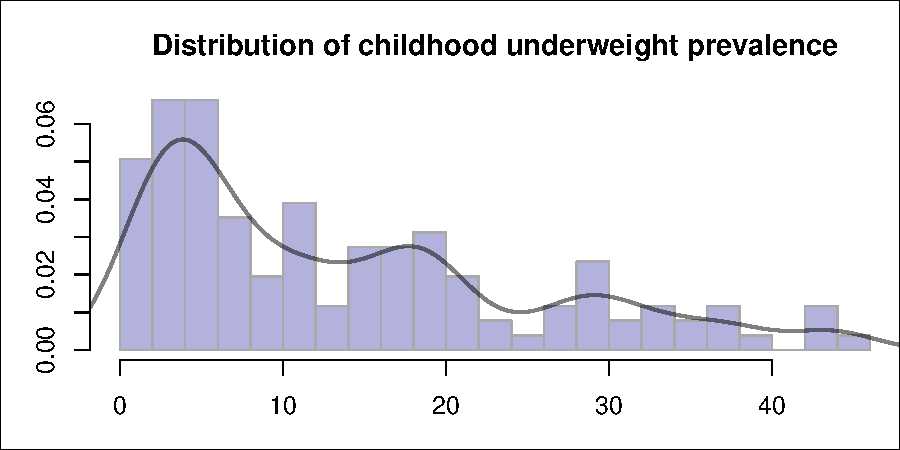
\includegraphics{global_variance-004}
\end{center}

%------------------------------------------
\subsection*{Breakdown by region}
\addcontentsline{toc}{subsection}{Breakdown by region}
%------------------------------------------

When country-level data are aggregated at the WHO administrative region level, two important characteristics stand out: variance between regions and variance within regions (see below).

\begin{center}
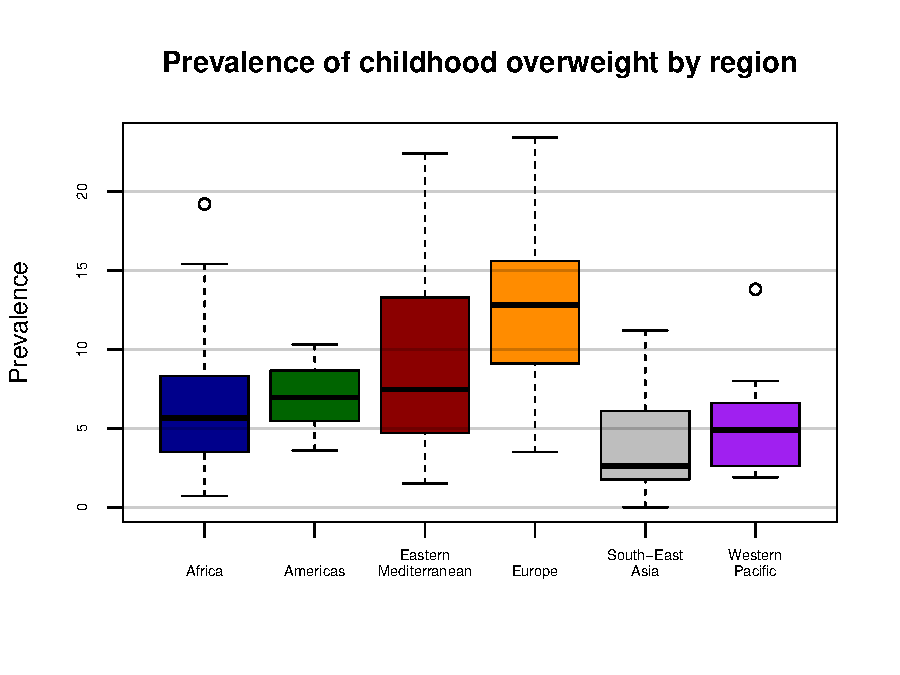
\includegraphics{global_variance-005}
\end{center}
%------------------------------------------
\subsection*{Breakdown by country}
\addcontentsline{toc}{subsection}{Breakdown by country}
%------------------------------------------

Breaking down the prevalence further (by country) sheds further light on the inter-region variance.  The below chart reveals some obvious trends (dark blue African countries are clustered to the left, whereas orange and red European countries are mostly to the right), but the take-away message is clear: variation is the norm. \\

\begin{center}
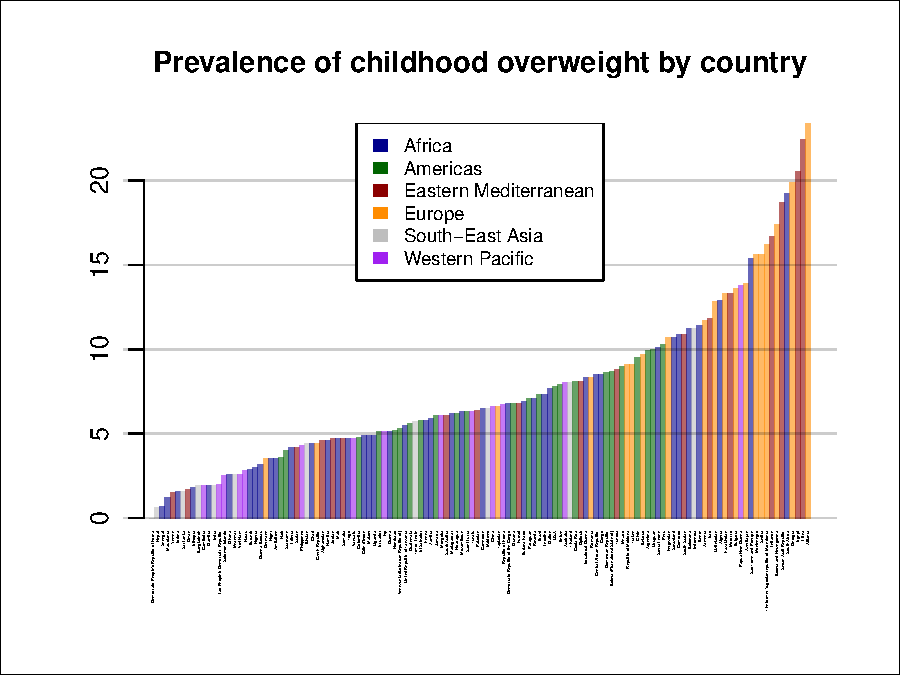
\includegraphics{global_variance-006}
\end{center}

%------------------------------------------
\subsection*{Breakdown by geography}
\addcontentsline{toc}{subsection}{Breakdown by geography}
%------------------------------------------
Mapping childhood obesity (ages 2-4) yields interesting findings, as it does not take the same pattern that later childhood obesity or adult obesity.  This could be anomalous; or, it could be a sign of rapid changes taking place.  In other words, the "hotspots" in Northern and Southern Africa may be in for an increasingly severe adult obesity epidemic in coming years.

\begin{center}
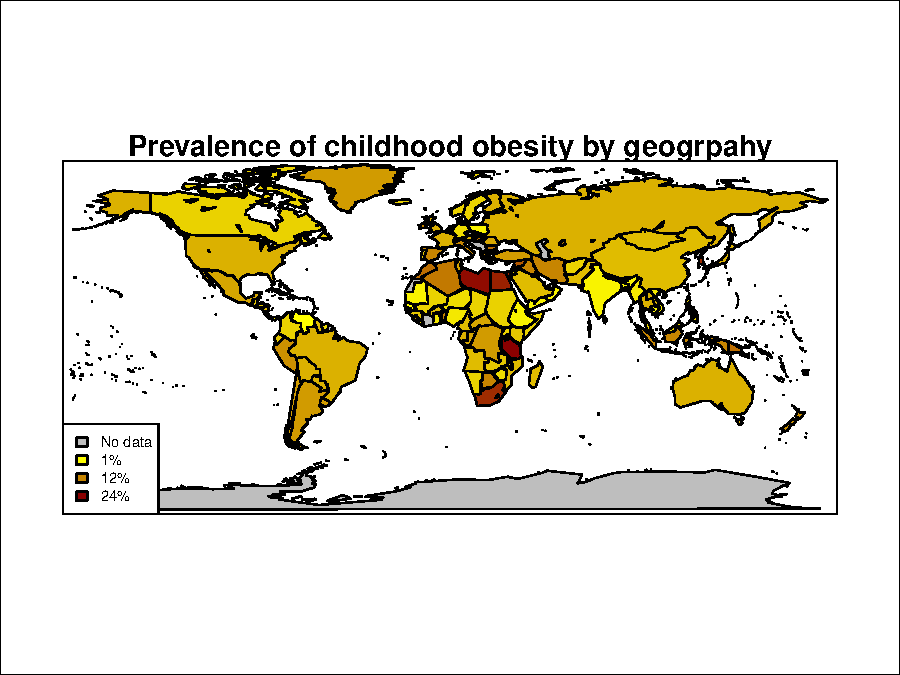
\includegraphics{global_variance-007}
\end{center}


%------------------------------------------
\subsection*{Correlations}
\addcontentsline{toc}{subsection}{Correlations}
%------------------------------------------

Using IMF data, once can compare the prevalence of childhood obesity to a country's GDP (gross domestic product) per capita (next chart).\\

\begin{center}
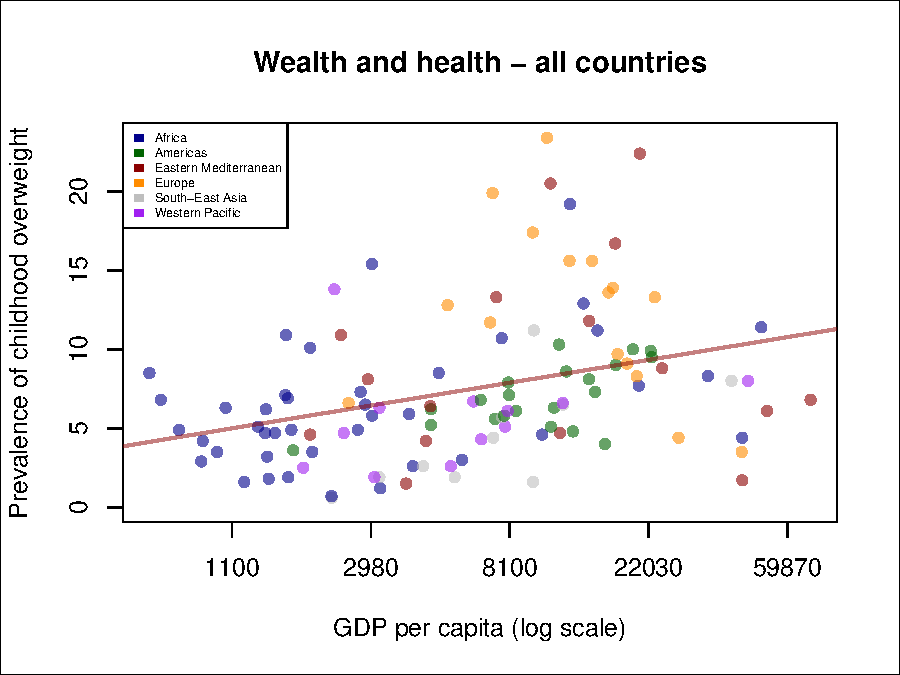
\includegraphics{global_variance-008}
\end{center}
What emerges is clearly a semi-linear relationship between a country's wealth and the prevalence of obesity (line of best fit using least squares method shown in red) (R-squared of approximately 0.11).  \\

However, more careful examination suggests that analysis at such a macro scale masks region-level differences in the relationship between wealth and health.  In other words, the effect of GDP per capita on childhood obesity changes in both magnitude and direction when analyzed at the regional level.  The below plot shows the line of best fit for each WHO region.  What is striking is that (western) Europe seems to have an inverse relationship between wealth and childhood obesity, unlike all the other regions.      \\

\begin{center}
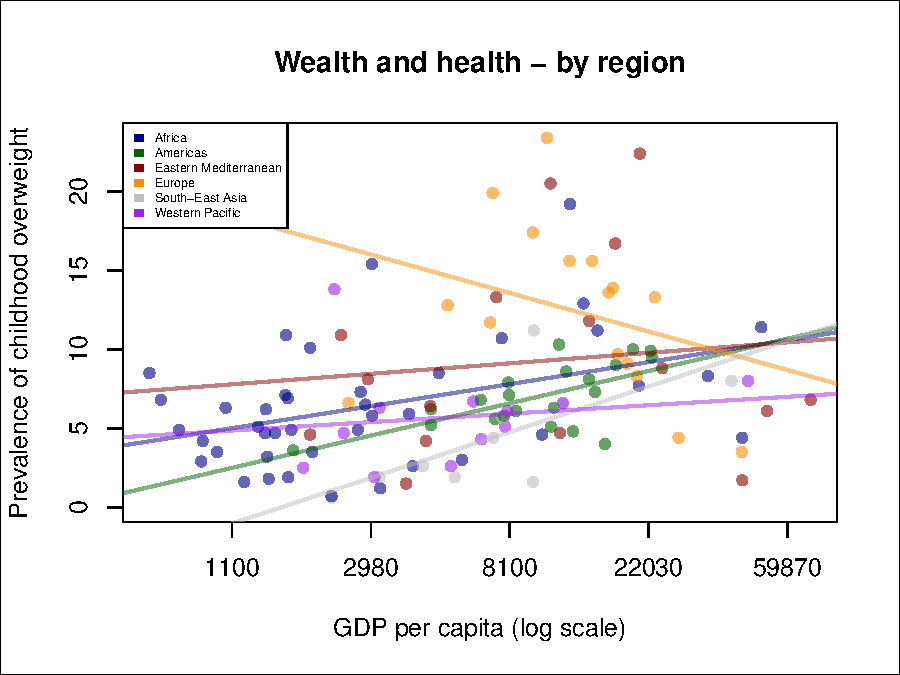
\includegraphics{global_variance-009}
\end{center}

When the interaction terms between region and GDP per capita / childhood obesity are introduced into a linear model, R-squared increases to 34\%.  In other words, the pathways to childhood obesity are likely different in different places.

%------------------------------------------
\subsection*{Conclusion}
\addcontentsline{toc}{subsection}{Conclusion}
%------------------------------------------

\noindent \textbf{Summary:} The prevalence of childhood obesity varies by region and country, and the magnitude and direction of the relationships between obesity and covariates (like wealth) also vary by country.  This is an important finding in that it confirms obesity's \emph{multi-causality}, and suggests that from an intervention standpoint a one-size-fits-all approach will likely be met with varying degrees of success. \\

\noindent \textbf{Limitations:} For this analysis, I only used the prevalence of overweight among 2 to 4 year-olds.  I also wrote a "fuzzy" matching algorithm to merge the data between OECD, WHO and IMF sources, which is prone to errors and mismatches.\footnote{Basically, if a country's name resembled a name in a different dataset, I considered it a match.   Full code is available at \url{https://github.com/joebrew/uf/tree/master/phc6016/assignment4}}  Finally, the estimates herein vary in both quality of data as well as time of collection.  \\

\noindent \textbf{Sources:} I used only data which is publicly available online.  
\begin{itemize}

\item IMF: \url{http://www.imf.org/external/pubs/ft/weo/2014/02/weodata/weorept.aspx}
\item OECD: \url{http://stats.oecd.org/index.aspx?DataSetCode=HEALTH_STAT}
\item WHO: \url{http://apps.who.int/gho/data/view.main.2450?lang=en}

\end{itemize} \\

\vspace{3mm}
\noindent \textbf{Technical details:} Figures are small, but will retain quality under zoom.  \\
All analysis, charts and maps were carried out entirely inR.  Code available at \url{https://github.com/joebrew/uf/tree/master/phc6016/assignment4}.    



\vfill
\columnbreak


%------------------------------------------
\subsection*{Other figures (just for fun)}
\addcontentsline{toc}{subsection}{Other figures (just for fun)}
%------------------------------------------


\begin{center}
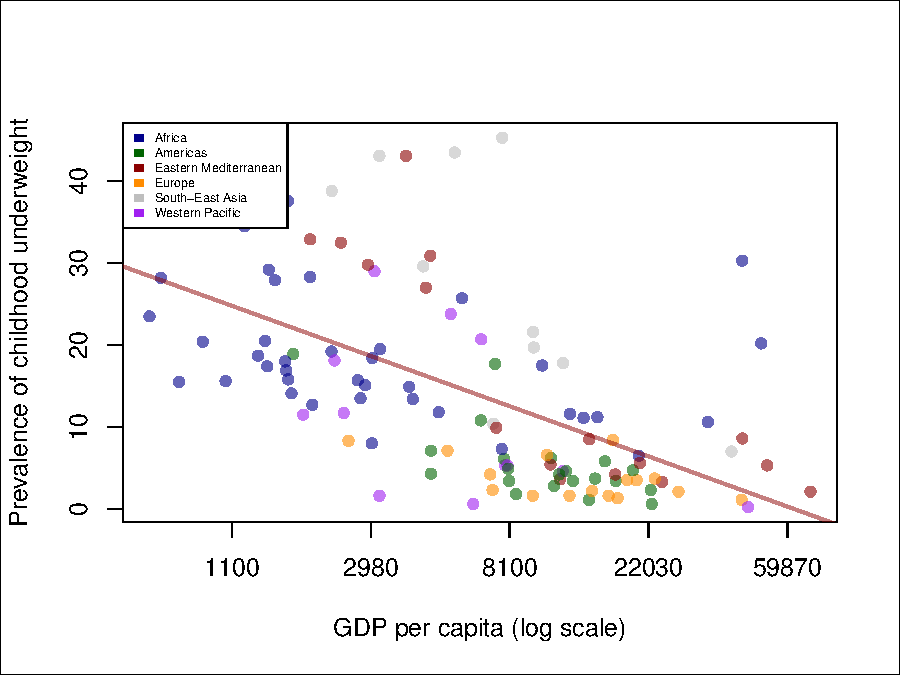
\includegraphics{global_variance-010}
\end{center}
\vspace{2mm}




\begin{center}
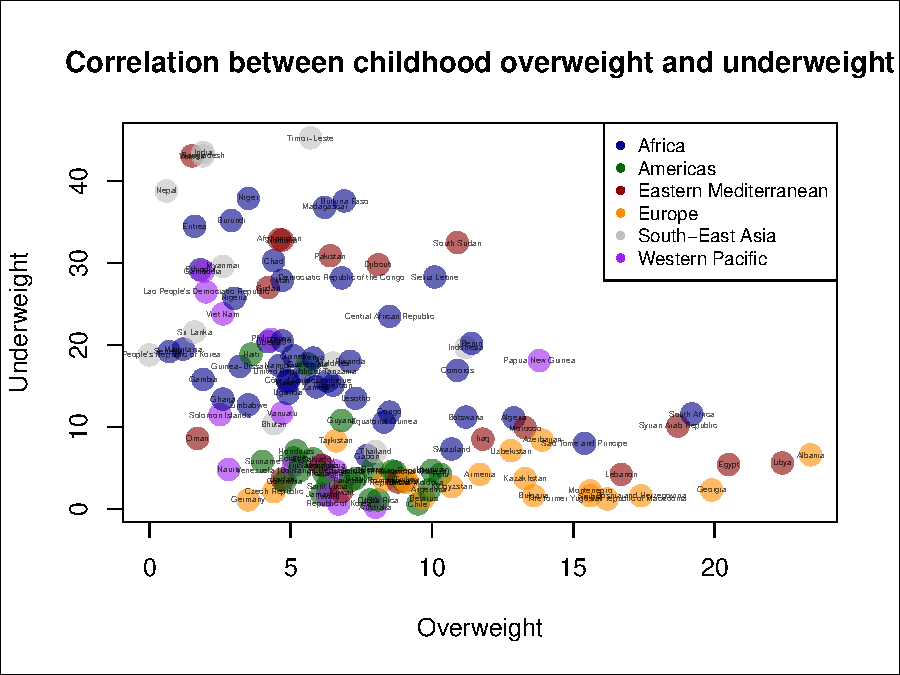
\includegraphics{global_variance-011}
\end{center}




\end{multicols}
\setkeys{Gin}{width=1\textwidth}
%----------------------------------------------------------------------------------------
%  REFERENCE LIST
%----------------------------------------------------------------------------------------
\newpage
\bibliographystyle{unsrtnat}
\bibliography{test}


\end{document}
